% !TEX root = ../my-thesis.tex
%
\chapter{Place du rehaussement de vaisseaux dans la segmentation}

% TODO : S'assurer que les différentes catégories scientifiques sont là
% TODO : Vérifier qu'il y a bien une justification vers un choix de progression et des parties dé-corélées sans fil conducteur.

\cleanchapterquote{Un petit chapitre pour le doctorant, un grand chapitre pour l'humanité}{Doctorant anonyme}{(Citation temporaire)}

\section{Problématiques}
    \subsection{Visualisation}

    Nous avons vu dans le chapitre précédent les différentes méthodes d'acquisitions ainsi que les différentes bases de données publiques disponibles. Après l'acquisition se pose la question de la visualisation des données. Le problème initial des médecins est en effet de détecter des anomalies visibles dans les images qui sont liées à des pathologies. La première méthode d'analyse, encore beaucoup utilisée aujourd'hui, est la visualisation des coupes 2D. À la manière de la TM ou de l'IRM, le médecin visualise l'image tranche par tranche. Elle nécessite toutefois de l'entrainement, puisque le médecin doit effectuer une gymnastique mentale pour reconstituer dans leur esprit les éléments en volumes \ref{fig:slice_visualization}. 

    \begin{figure}[t!]
      \centering
      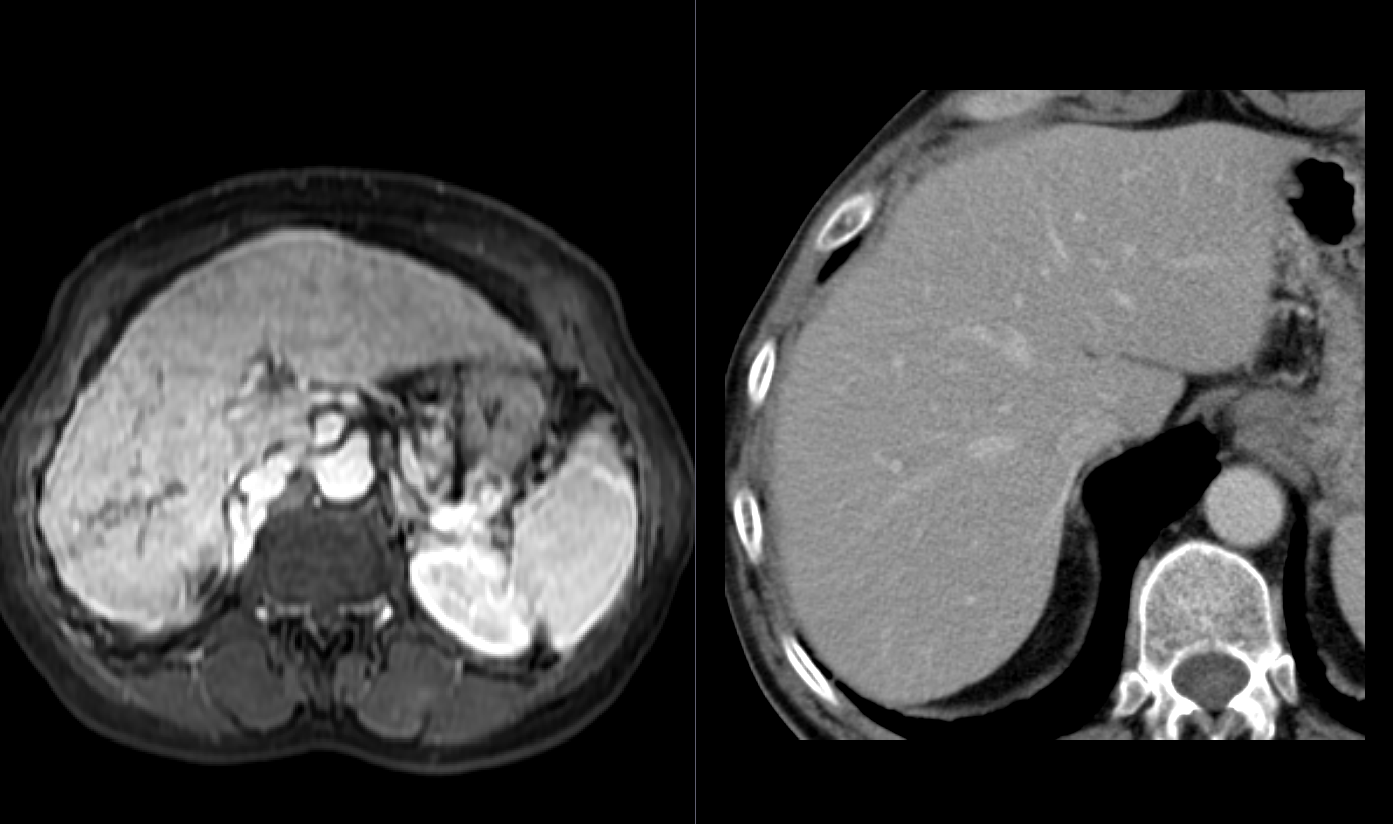
\includegraphics[height=5cm]{Images/2D_view.png}
      \caption{Visualisation en coupe, à gauche IRM, à droite tomodensitométrie}
      \label{fig:slice_visualization}
    \end{figure}

    La visualisation en 3D, qui consiste à considérer l'ensemble des coupes comme un volume 3D facilite cet exercice. Elle permet ainsi de visualiser directement les structures dans leur entièreté. On peut distinguer deux manières de visualiser les données. Une première méthode où l'on se contente de projeter les données existantes dans un plan particulier et une seconde manière où l'on extrait les structures d'intérêts.

      \subsubsection{MIP}
      La MIP (Maximum Intensity Projection) est une technique de projection permettant de visualiser les éléments les plus saillants d'une image. En pratique, elle consiste à créer un plan image 2D $P$ puis pour chaque pixel $p_i$ de ce plan de lancer un rayon qui traverse le volume 3D. Pour l'ensemble des voxels qui intersectent le rayon, on récupère la valeur maximale parmi leur intensité que l'on affecte à $p_i$ (Fig. \ref{fig:MIP_visualisation}). 

      \begin{figure}[h]
        \centering
        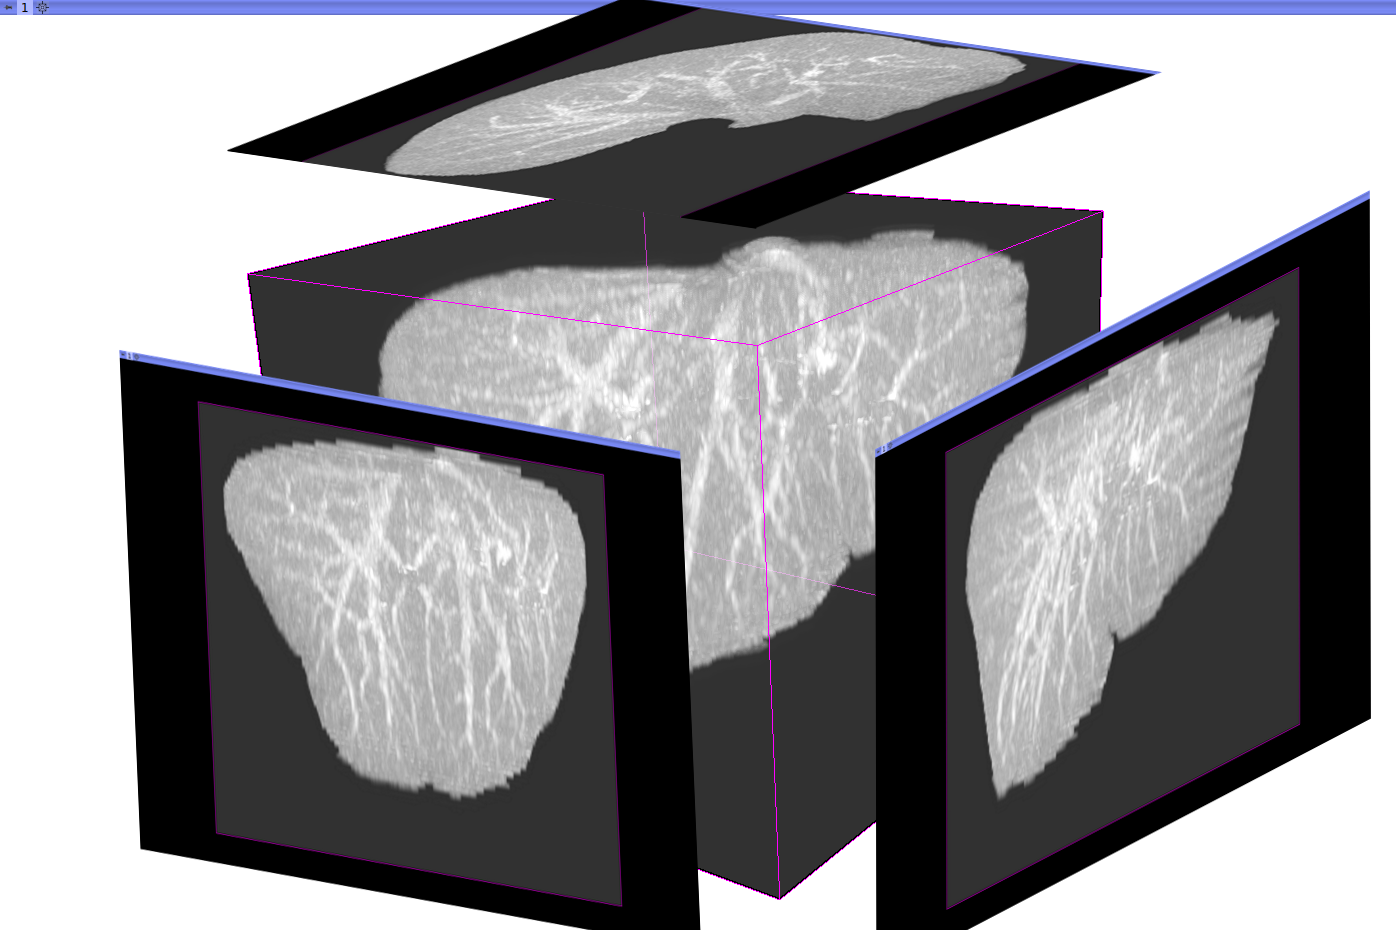
\includegraphics[height=5cm]{Images/3D_mip_montage.png}
        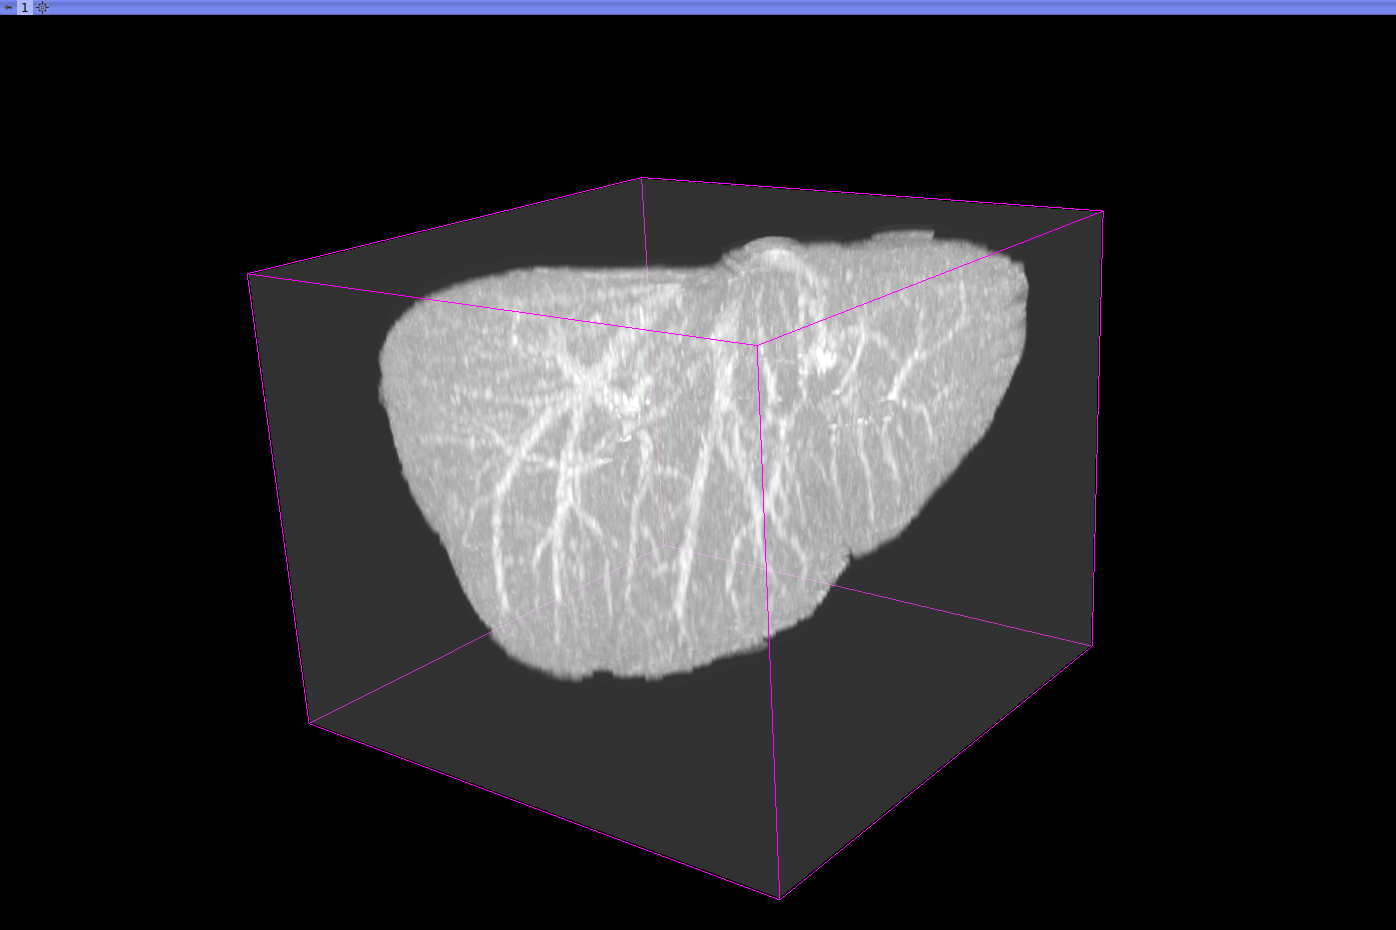
\includegraphics[height=5cm]{Images/3D_mip.png}
        \caption{Maximaly intensity projection. L'intensité maximale est rétro-projeté le long du rayon sur le plan d'origine. La MIP peut s'effectuer en utilisant les bords de l'image, où le plan de la caméra dans une scène 3D}
        \label{fig:MIP_visualisation}
      \end{figure}

      Cette méthode permet de faire ressortir les éléments les plus intenses de l'image et convient particulièrement à des structures mises en valeur par agent de contraste. Elle est simple à implémenter et peu coûteuse en calcul. Elle fait cependant perdre toute perception de profondeur par la projection des maximums sur le plan image. Par exemple, une MIP dont les rayons traversent le dos puis le ventre produit la même image (à effet miroir prêt) qu'une MIP avec des rayons traversant le ventre puis le dos. La perte de profondeur se compense lorsque dans un scène 3D, le plan de projection devient le plan de la caméra. Le mouvement de la caméra permet alors de résoudre les ambiguïtés provoquées par un seul plan de projection. 
      La MIP a aussi le désavantage d'être parasitée par toutes structures plus intenses que l'organe observé. L'observation du foie et de ses vaisseaux en MIP est donc perturbée par les os de la cage thoracique. Ce problème peut cependant être contourné en appliquant un masque pour ne conserver que le foie, ce qui demande un coût supplémentaire d'annotations.

      \subsubsection{Segmentation}
      
      D'autres moyens de visualisation sont possibles, par exemple en représentant un modèle 3D des structures observées. On peut ainsi visualiser des organes seuls, sans éléments adjacents perturbateurs. La création de ce modèle nécessite un traitement plus complexe des données afin d'identifier, de classer, de filtrer puis d'extraire les structures d'intérêts. C'est ce processus que l'on nomme la segmentation. Là où l'utilisation de la MIP est limitée dans ses usages, la segmentation a des champs d'applications plus larges comme la simulation ou l'extraction de données comme le volume et la géométrie d'un réseau vasculaire.
  
  \subsection{Amélioration des images}
      La littérature de l'imagerie médicale gravite autour de deux sujets principaux : l'amélioration de la qualité des images et les algorithmes de segmentation.

    \subsubsection{Amélioration du signal}
      
    Historiquement, le besoin d'améliorer la qualité des images provient des limitations des premières machines d'imagerie. Il était alors nécessaire de développer des méthodes efficaces pour limiter les artefacts tel que le bruit et de faire ressortir les organes d'intérêts. De nombreuses méthodes ont cherché à caractériser \cite{Gudbjartsson1995r_Rician_noise_MRI}, estimer \cite{Dietrich2007_measurement_MR_noise} \cite{Gravel_2004_estimate_noise_medical_img} puis corriger le bruit \cite{Krissian_2009_diffusion_MRI},\cite{Mendrik2009_HDCS}.

    De nos jours, les progrès techniques et l'amélioration de la résolution des machines ont résolu beaucoup de ces problèmes. Les algorithmes ont maintenant pour objectif de challenger les limites des machines, en termes de résolution. C'est par exemple le cas de méthodes à base de deep learning \cite{Higaki2019_deep_MRI_CT_quality} qui permettent d'améliorer la résolution et de corriger le bruit.

    \subsubsection{Extraction}
      Les algorithmes d'extractions sont souvent basés sur des algorithmes efficaces sur des photographies. La plupart sont formulées sous la forme d'un problème d'optimisation dans lequel on définit une énergie à minimiser. 
      
      \paragraph{Courbes de niveaux} La méthode des courbes de niveaux (level sets en anglais) permet de faire s'étendre un contour en fonction du temps, jusqu'à ce qu'un critère d'arrêt soit atteint. Ce critère peut reposer sur un modèle des structures à segmenter, des caractéristiques de l'image ou des propriétés sur la courbure du front de propagation du contour. Les courbes de niveaux sont une formulation implicite d'un contour exprimé comme l'intersection de deux surfaces. La première surface correspond à l'image vue comme une carte de hauteur et la seconde courbe $\phi$ correspond aux critère de partition (Fig. \ref{fig:level_set}). La dynamique d'évolution du contour implicite est géré par l'élévation de la courbe $\phi$ en fonction du temps. Ce mécanisme permet de contourner le problème du suivi du contour lorsque sa topologie change (i.e séparation en deux contours distincts).

      \begin{figure}[h]
        \centering
        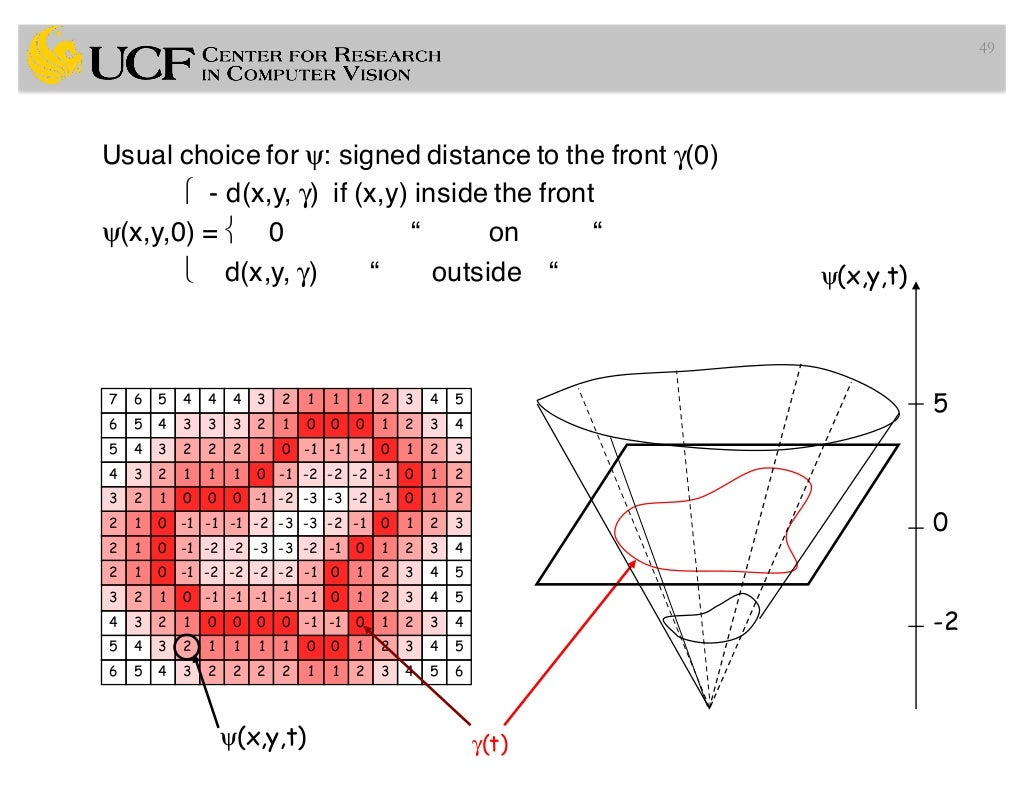
\includegraphics[height=4cm]{Images/level_set_active_contour.jpeg}
        \caption{Courbes de niveaux définissant un contour comme l'intersection de deux courbes implicites.}
        \label{fig:level_set}
      \end{figure}

      Par exemple, Li \cite{Li2011_mri_level_set} utilise les courbes de niveaux pour segmenter des objets malgré une intensité globale non homogènes, pour cela il définit un critère de classification local au voisinage des pixels afin d'estimer un champ de biais d'intensité qui est ensuite incorporé dans l'énergie de propagation. Une sous catégorie des courbes de niveaux est la méthode développée par Kass et al. \cite{Kass1988_snakes} des contours actifs (aussi appelés snake). Cette méthode formule l'énergie contrôlant la propagation du contour comme la somme pondérée d'une énergie interne et d'une énergie externe à minimiser. Cette énergie a ensuite connues de nombreuses variations comme Wang et al. \cite{Wang2012_vessel_level_set} qui propose un modèle minimisant 3 énergies : une énergie basée sur la courbure du contour, une énergie basée sur les gradients d'intensités de l'image et une énergie basée la correspondance du contour à un modèle cylindrique. Zeng \cite{Zeng2018_liver_hybrid_active_contour_region_growing} utilise les de contour actifs pour segmenter les gros vaisseaux, sans débordement des structures. La paramétrisation du contour actif est basé sur l'estimation de l'intensité des vaisseaux fins détectés par un filtre bi-Gaussien.

      \paragraph{Graph cut}
      Une image peut aussi être représentée sous la forme d'un graphe. Dans ce graphe, les nœuds sont les pixels et les arêtes encodent une relation de similarité entre les pixels. Cette relation peut être spatiale où plus complexe. Dans ce contexte, segmenter un objet ou une région revient à trouver la coupure qui maximise la vraisemblance à l'intérieur de chaque partition et minimise la vraisemblance entre deux partitions relativement à un critère (Fig. \ref{fig:graph_cut}).

      \begin{figure}[h]
        \centering
        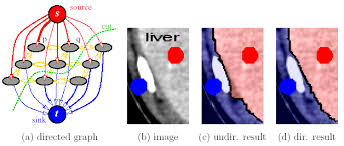
\includegraphics[height=4cm]{Images/graph_cut.jpeg}
        \caption{Principe du graph cut. Une partition est trouvée entre deux régions initialisées par une graine.}
        \label{fig:graph_cut}
      \end{figure}

      Esneault \cite{Esneault2009_moments_graph_cut} utilise afin de minimiser une énergie composée de 3 critères (région, bordure et vaisseaux). Le modèle de vaisseaux est basé sur un modèle cylindrique.

      Zeng \cite{Zeng2017_liver_oof_graph_cut} propose un raffinement d'une segmentation initiale par graph cut, en utilisant un critère de région basé sur la vraisemblance logarithmique (negative log likelyhood) et un critère de bordure basé sur le flux (voir Sec. Flux).

      \paragraph{Ensemble flou}

      Le choix d'une délimitation entre fond et segmentation n'est pas toujours aisé, en particulier dans les images médicales où les bords des objets à segmenter sont assez mal définis. La théorie des ensembles flous permet de modéliser cette incertitude. Au lieu d'associer une classe binaire aux pixels, on associe à chaque pixel une probabilité d'appartenance à chaque classe définie pour le problème donné. Un critère flou est ensuite construit afin de définir une segmentation binaire définitive.

      Sigurosson \cite{Sigurosson2014_retinal_morpho_fuzzy} utilise un ensemble flou pour la segmentation de vaisseaux dans la rétine. 

      Radojevic et al.\cite{Radojevic2015_fuzzy_logic} détecte les neurones en proposant deux classes floues basées sur le concepte de classes multiplicatives. Il définit ensuite le degré d'ambiguïté d'un ensemble flou afin d'attribuer une classe finale aux pixels.
      Zhang et al. \cite{Zhang2018_liver_fuzzy_connectedness} définit un critère de connectivité floue composé d'un critère d'adjacence floue des voxels, et un critère de similarité à la géométrie d'un vaisseau basé sur les filtres de rehaussement de vaisseaux.  


      \paragraph{Deep learning}

      % Better results with deep learning
      Dans les années 2010, un changement de paradigme a lieu avec l'utilisation croissante des réseaux de neurones. En effet, l'apparition des modèles de réseaux profonds, de l'augmentation de la puissance de calculs et d'un nombre important de données annotées ont drastiquement augmenté les performances de ces modèles.

      À partir de 2015, les réseaux de neurones, et en particulier les réseaux convolutifs (CNN) ont pris une place prépondérante dans la littérature de la segmentation grâce à l'apparition des modèles de réseaux profonds, de l'augmentation de la puissance de calculs et d'un nombre important de données annotées.

      En pratique, on fournit des exemples à un réseau qui produit en réponse une prédiction. L'erreur entre la prédiction et la vérité terrain est ensuite rétro-propagée dans le réseau afin qu'il puisse corriger les prédictions erronées. Ce processus, appliqué de manière itérative sur un grand nombre d'exemples, est appelé entrainement. Deux types d'entraînement sont principalement utilisés, l'entraînement supervisé par paires \{image d'entrée, vérité terrains\} et l'entraînement non supervisé avec des images en entrée et une énergie à minimiser qui permet de contraindre la prédiction du réseau.
      % what is used in medical applications
      Dans le milieu médical, ce sont les réseaux convolutifs complets (FCNN), en particulier l'architecture d'auto-encodeur U-Net \cite{Ronneberger2015_Unet}, qui se sont imposés en permettant de segmenter de manière précise des organes. Ce modèle propose une architecture composée d'un encodeur et d'un décodeur symétriques, donnant au réseau sa forme en U caractéristique. Des ``skip connections'', permettent de propager les détails de l'encodeur au décodeur.

      Un large panel de variantes de ce réseau a été proposé dans la littérature, combinant ResNet \cite{yu2019_liver_ResUnet}, DenseNet \cite{Li2018_DenseUnet}, en utilisant plusieurs réseaux travaillant à des résolutions différentes ou en proposant des branches spécialisées.
      % Loss
      Les résultats des réseaux de neurones sont très dépendants de la fonction de coût qui évalue l'erreur entre la prédiciton et les données. Pour la segmentation, la ``Dice loss'' proposée par Sudre \cite{Sudre2017_DiceLoss} s'est popularisée. Cette fonction de coût repose sur le Dice qui mesure le recouvrement entre la prédiction et la vérité terrain. Plusieurs métriques similaires ont été proposée et une revue des fonctions de coût pour la segmentation est proposé par \cite{Jadon2020_survey_seg_loss}. Plus récemment des travaux ont exploré l'introduction de critères topologiques (composantes connexes) afin de limiter la fragmentation des segmentations, particulièrement pertinent pour les structures fines comme les vaisseaux \cite{Hu2019_topo_homo_persi},\cite{Clough2019_topo_homo_persi},\cite{Ventura2017iterative_topo}. Ces méthodes restent toutefois très coûteuses en temps. 
      % Data
      Le nombre des données joue un rôle crucial dans la performance des réseaux de neurones. Cependant, nous avons vu dans le Chap. 2 les difficultés de trouver des bases de données publiques avec un nombre important de données et bien annotées. 

      Plusieurs méthodes permettent de contourner partiellement ce problème. La plus utilisée est l'augmentation de données, \cite{Liskowski2016_data_augmentation}. Celle-ci utilise des données existantes pour appliquer des changements d'intensités ou des déformations géométriques afin de créer artificiellement des données supplémentaires.

      D'autres méthodes comptes sur l'utilisation de données partielles, ou d'annotations complètes sur seulement une partie des données \cite{Tajbakhsh2020_imperfect_datasets}. Certains auteurs ont exploré le transfert de style afin de générer des images d'une modalité grâce à des images d'autres modalités. Chartsias et al. \cite{Chartsias2017_heart_adversarial_im} propose la génération adversaire d'images IRM grâce à des images CT et un masque d'alignement des structures. Chartsias montre qu'en entraînant un réseau sur des images réelles et synthétiques, on augmente les performances d'un réseau de segmentation. Huo et al. \cite{Huo2018_adversarial} explore la génération à la fois d'une nouvelle modalité et de sa segmentation.

    \subsubsection{Problématiques de la segmentation}

    Créer une chaîne de segmentation est une tâche complexe. Elle doit apporter des réponses efficaces à la fois à la gestion des artefacts d'acquisition des images, de l'apparence des organes à détecter et de l'extraction d'éléments sémantiques de haut niveau. 

    Les solutions ont été apportées par l'élaboration de chaines de traitements complexes pour les méthodes sans deep learning. Ainsi, pour la segmentation des vaisseaux hépatiques, Marcan \cite{Marcan2014_vessel_seg} propose un pipeline de segmentation en 16 étapes mélangeant, filtrage du bruit, sélection des éléments pertinents par masques et analyses des composantes connexes pour la segmentation des vaisseaux du foie. Goceri \cite{Goceri2017_vessel} propose une méthode en 14 étapes alliant partions en régions d'intérêts et étirement du contraste (contrast stretching) afin de différencier vaisseaux hépatiques des tissus du foie.
  
    Pour le deep learning, cette complexité se situe au niveau de la construction de l'architecture du réseau et de la construction de la base de donnée. Si l'on veut traiter l'information en 3D afin de tirer partie de l'ensemble de la géométrie des vaisseaux, les ressources physiques nécessaires deviennent rapidement un goulot d'étranglement.  
    
    Malgré une littérature dense pour la segmentation vasculaire, illustrée dans les revues de Lesage et al. \cite{Lesage2009_review}, Tankyevych et al. \cite{Tankyevych2011_angiographic} et Moccia et al. \cite{Moccia2018_survey} il n'est pas facile de juger de l'efficacité d'une méthode de segmentation par rapport à une autre. Cette difficulté s'illustre dans les tableaux comparatifs de l'état de l'art conduit par  Moccia (Fig. \ref{fig:custom_fig}) qui montre plusieurs problèmes.

    \begin{figure}[h]
      \centering
      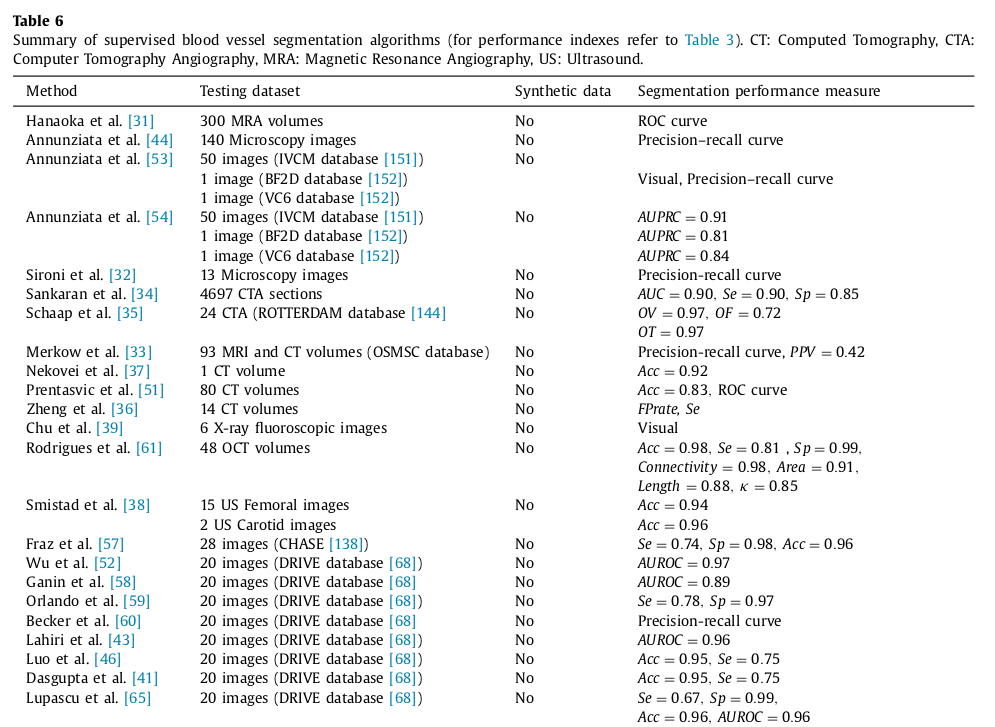
\includegraphics[height=6cm]{Images/Moccia_example.png}
      \caption{Table partielle tirée de Moccia et al. \cite{Moccia2018_survey} récapitulant les résultats de différentes méthodes de modèles déformables. Elle illustre la diversité des jeux de données et des méthodes d'évaluations.}
      \label{fig:custom_fig}
    \end{figure}

    Premièrement, il y a disparité dans les métriques de comparaisons. Certains articles utilisent les métriques standard de classification : précision, accuracy, sensibilité, spécificité. d'autres articles utilisent des métriques de recouvrement comme le Dice ou les coefficients de corrélations de Matthew (MCC) et d'autres des opérateurs intégraux de type AUC, ROC. Les résultats de certaines méthodes sont mêmes parfois évalués visuellement par des experts.

    Deuxièmement, il y a une disparité dans les jeux de données. Entre deux articles, il peut y avoir de grandes différences sur le nombre d'images utilisées, les modalités d'acquisition et leur disponibilité. Cette disparité est plus marquée pour les volumes 3D. Des contre exemples existent comme pour l'imagerie du fond de l'oeil (fundus) qui disposent de 3 jeux de données annotés qui font référence. L'accessibilité de ces jeux de données annotés est en partie responsable du grand nombre d'articles les utilisant.

    Troisièmement, il est difficile de juger les bénéfices de chaque bloc algorithmique dans une chaine de segmentation. Une étude ablative où chaque bloc est remplacé afin d'étudier sa performance, comme on pourrait le faire sur les de réseaux de neurones n'est pas forcément possible. Il est donc complexe de juger si les gains obtenus par une méthode sont obtenus grâce à sa modélisation du problème, l'utilisation de caractéristiques particulièrement pertinentes ou de la métrique permettant une segmentation efficace.

    En étudiant plus en détail les blocs algorithmiques utilisés pour la segmentation vasculaire traditionnelle, une famille de filtres est utilisée régulièrement en amont des chaines de traitement. Leur positionnement en fait un élément clés qui conditionnent la suite de la segmentation. Ces filtres ont aussi la possibilité d'être appliqués sur les données d'entrées pour le deep learning. Une étude de leurs propriétés nous paraissait donc pertinent comme un premier pas vers la construction d'un algorithme de segmentation.


  \section{Modélisation}

  Les filtres de rehaussement cherchent à isoler et améliorer le signal des structures géométriques associées à des vaisseaux (Fig. \ref{fig:exemple_vesselness}). Ces filtres répondent en tout ou partie aux objectifs suivants :

  \begin{itemize}
  \item Détecter les structures vasculaires.
  \item Différencier les structures vasculaire des autres structures.
  \item Filtrer les autres structures afin de ne garder que les vaisseaux.
  \item Améliorer le signal des vaisseaux
  \end{itemize}

Les filtres de rehaussement de vaisseaux reposent sur quatre concepts : La modélisation des vaisseaux, le type de caractéristiques utilisées, l'espace d'échelle et la mesure de similarité par rapport au modèle. La modélisation la plus populaire est d'assimiler les vaisseaux à des structures tubulaires. En effet, les vaisseaux sont de longues structures pleines et tortueuses dont la géométrie varient de la ligne (1 voxel de diamètre) à des tronçons de périmètres irréguliers. Les réseaux vasculaires sont formés par la connection de structures tubulaires qui forment alors une bifurcation. On parle de  bifurcations quand un vaisseau principal se divise en deux sous vaisseaux, trifurcations en trois et N-furcations dans le cas général. Dans la suite de ce manuscript, nous effectuons un abus de langage en appelant "bifurcations" l'ensemble des furcations, puisque c'est le cas le plus courament rencontré. Des hypothèses sont aussi faites sur l'intensité des vaisseaux. Selon les modalités, les vaisseaux peuvent apparaitre noirs sur fond plus clairs (IRM en phase T1, angiograme) ou blanc sur fond plus foncé (IRM en phase T2, injection d'agent de contraste). Les hypothèses sont interchangeables, car on peut tout à fait inverser les niveaux de gris de l'image pour passer d'une hypothèse à l'autre. Pour la suite, nous prenons l'hypothèse que les vaisseaux sont clairs sur fond plus sombre.

\begin{figure}[h]
  \centering
  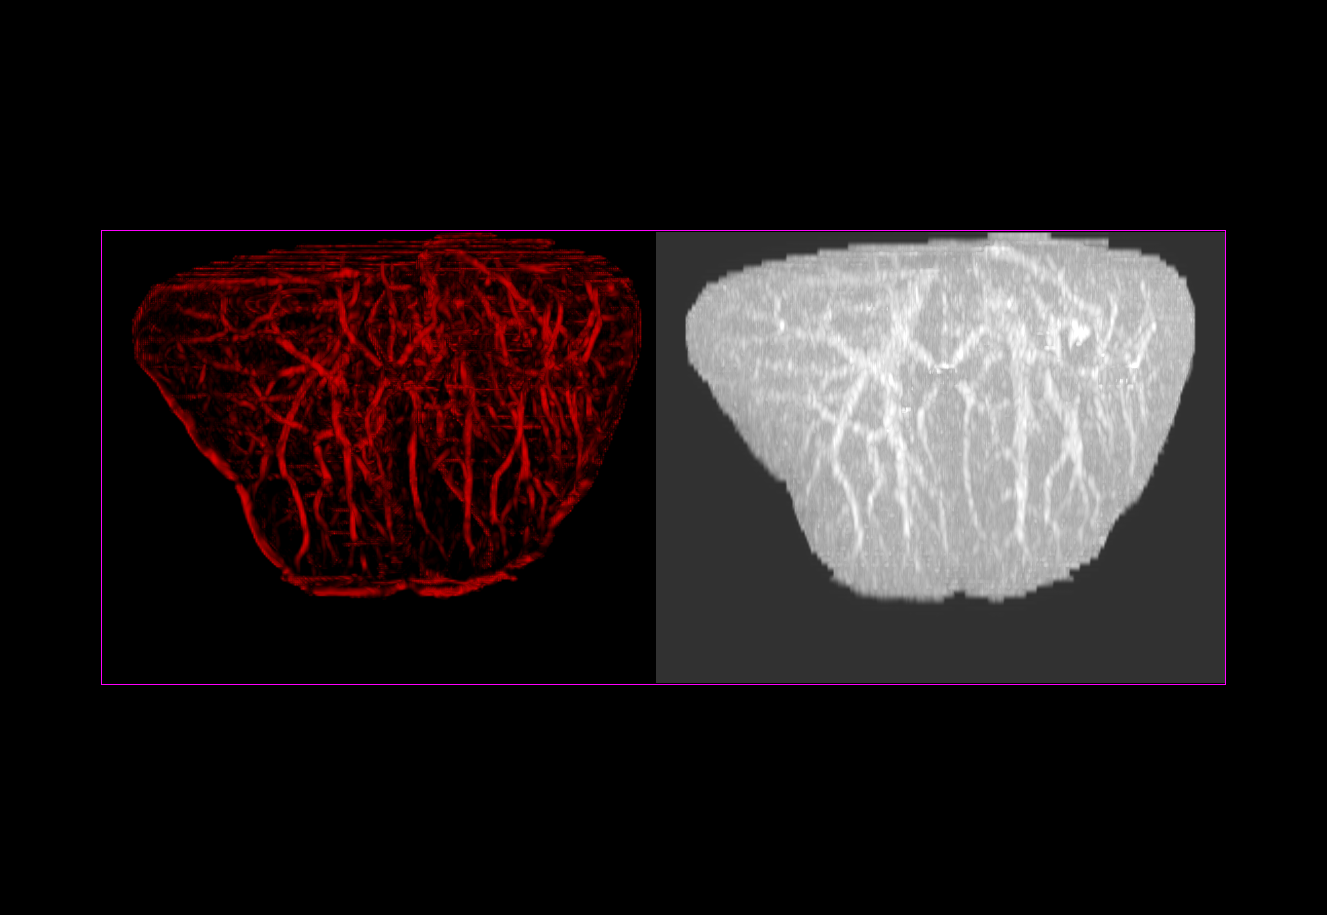
\includegraphics[height=5cm]{Images/vessels_enhancement.png}
  \label{fig:exemple_vesselness}
  \caption{exemple de filtre de rehaussement de vaisseaux. À droite, un foie en MIP, à gauche les vaisseaux rehaussés. La plupart des vaisseaux sont conservés, ainsi que des artefacts de bruit et de bordure. }
\end{figure}

  Avant de définir les caractéristiques utiles à la détection de structures tubulaires, il est nécessaire de définir un espace dans lequel on peut représenter des vaisseaux de tailles différentes dans un cadre commun.

  \section{Espace d'échelles}
  \label{sec:EA:rehaussement:echelle}
  
  La détection d'un réseau vasculaire dans sa totalité implique de détecter des vaisseaux de différentes tailles. En effet, les plus gros vaisseaux peuvent faire plusieurs dizaines de voxels de diamètres tandis que les vaisseaux les plus fins, atteignant les limites de la résolution des capteurs, peuvent  mesurer jusqu'à un voxel de diamètre. Il n'est pas envisageable de réécrire un algorithme pour chaque taille de vaisseaux, c'est pourquoi des cadres théoriques, appelés \emph{espace d'échelle} ont été formulés. Ces espaces d'échelles permettent d'établir un cadre uniforme pour sélectionner les structures d'une image à une échelle donnée. Trois espaces d'échelles sont couramment associés au rehaussement de vasculaire dans la littérature : L'espace d'échelle gaussien, l'espace d'échelle granulométrique et l'espace d'échelle de flux orienté.
  
  \subsection{Espace Gaussien}
  \label{sec:EA:rehaussement:echelle:gaussien}
  
  Lindenberg introduit la théorie de l'espace d'échelles gaussien dans \cite{Lindeberg2013_scale}. Dans cette théorie, a l'échelle la plus basse, la totalité des structures sont présentes et les détails les plus fins sont présents. Au fur et à mesure que l'échelle augmente, les détails sont lissés pour ne laisser que les maxima locaux correspondants aux formes les plus grandes. Ainsi, l'échelle minimale correspond à l'image initiale et l'échelle maximale correspond à une image uniforme (Fig. \ref{fig:gaussian_smoothing} ). Lindenberg a aussi montré que les noyaux Gaussien étaient les seuls noyaux permettant de passer d'une échelle fine à une échelle grossière sans provoquer l'apparition de nouvelles structures. De plus, un fonctionnement identique a été observé dans le fonctionnement de la vision humaine.
  
  \begin{figure}[h]
    \centering
    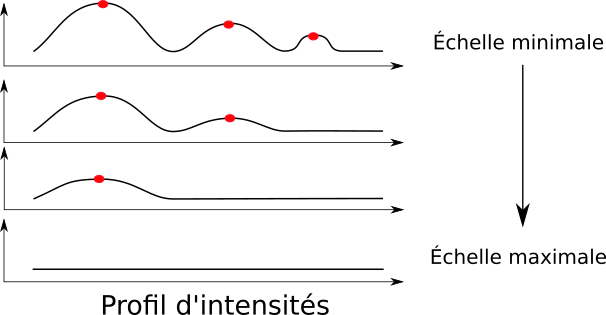
\includegraphics[height=5cm]{Images/gaussian_smoothing.png}
    \label{fig:gaussian_smoothing}
    \caption{Lissage gaussien, les structures de taille égales ou supérieures à $\sigma$ sont conservées alors que les structures de taille inférieures disparaissent}
  \end{figure}
  
  \begin{equation}
    gauss(x,y,\sigma_{x},\sigma_{y}) = \frac{1}{ \sigma\sqrt{2\pi} }exp(-\frac{x^2 + y^2 + z^2}{2(\sigma_{x}+ \sigma_{y}+ \sigma_{z}) })
    \label{eq:Gaussienne 3D}
  \end{equation}
  
  La sélection de l'échelle dans un espace gaussien se fait par le choix de l'écart-type $\sigma$ de la gaussienne (Fig. \ref{fig:normal_distribution_probability_coverage}). La plupart du temps on considère un espace d'échelle uniforme, $\sigma_x = \sigma_y = \sigma_z$. Il faut noter que pour un $\sigma$ donné, la taille des structures n'est pas supérieure ou égale à $\sigma$, mais plutôt supérieure ou égale à $\alpha\sigma$. En effet, en empruntant le formalisme des statistiques, l'intervalle de confiance, c'est-à-dire la couverture d'une distribution normale, correspond à $34.1$ pourcent pour $\sigma=1$, $68$ pourcent pour $\sigma=2$ et $99.7$ pourcent pour $\sigma=3$. Ainsi, pour $\sigma=1$ on détectera en théorie des objets de rayon $3\sigma$ et de diamètre $6\sigma$.  
  
  \begin{figure}[h]
    \centering
    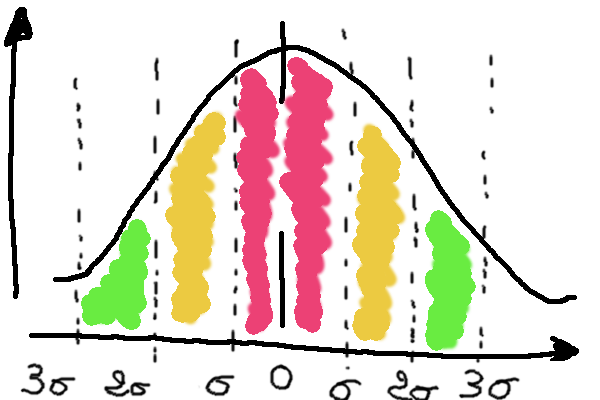
\includegraphics[height=5cm]{Images/normal_distribution_probability_coverage.png}
    \label{fig:normal_distribution_probability_coverage}
    \caption{couverture d'une distribution normale}
  \end{figure}
  
  L'espace gaussien se prête particulièrement bien à la modélisation des vaisseaux. En effet, la formulation de la gaussienne correspond bien à l'effet combiné des hypothèses de vaisseaux cylindriques et des observations de la diminution d'intensité des vaisseaux au fur et à mesure que l'on s'éloigne de leur centre. En particulier pour un vaisseau parfait de diamètre $3\sigma$, les maxima locaux se situent le long de sa ligne centrale.
  
  De plus, la gaussienne se prête très bien à une analyse locale de la géométrie basée sur la dérivation. Elle assure en effet les hypothèses de continuité du support de l'image et permet de combiner lissage et dérivation de l'image en une seule étape par dérivation du noyau gaussien.
  
  Enfin, le lissage a l'avantage d'apporter une certaine robustesse au bruit et de compenser la perte locale de signal.
  
  L'espace gaussien a toutefois des défauts. Le lissage de l'image implique nécessairement un étalement de toutes les structures qui peuvent par conséquent cacher des structures voisines de plus petites tailles. Ce phénomène est particulièrement observé lorsque plusieurs échelles sont étudiées. De même, deux structures adjacentes de même taille peuvent fusionner, et ainsi créer une seule réponse, là où deux objets existaient initialement (Fig. \ref{fig:scale_space_spilling}).
  
  \begin{figure}[h]
    \centering
    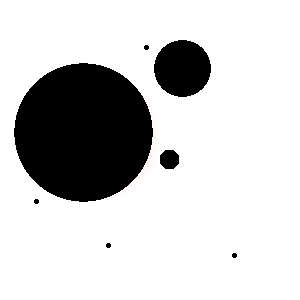
\includegraphics[height=3cm]{Images/gaussian_spilling_init.png}
    
\includegraphics[height=3cm]{Images/gaussian_spilling_g10.png}
    
\includegraphics[height=3cm]{Images/gaussian_spilling_g40.png}
    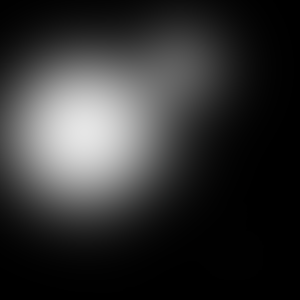
\includegraphics[height=3cm]{Images/gaussian_spilling_g100.png}
    \label{fig:scale_space_spilling}
    \caption{Débordement du signal des structures larges sur les structures de plus petite taille}
  \end{figure}
  
  \begin{figure}[h]
    \centering
    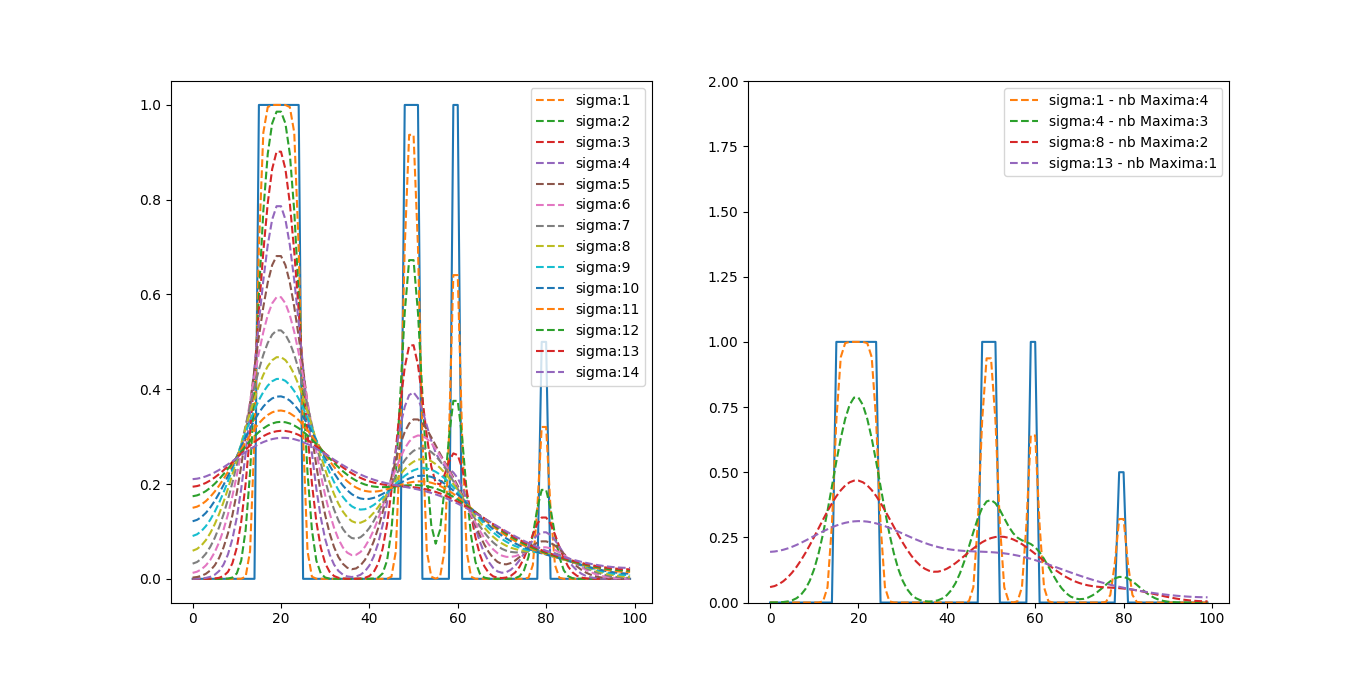
\includegraphics[height=5cm]{Images/GSP_experiment.png}
    \label{fig:scale_space_spilling2}
    \caption{Effet du lissage sur les structures en fonction de $\sigma$. Deux phénomènes sont observés, la fusion et le déplacement des pics des structures adjacentes. Le lissage fait disparaître les structures de faible intensité ou trop fines.}
  \end{figure}
  
  
  
  \subsection{Granulométrie}
  \label{sec:EA:rehaussement:echelle:granulometrie}
  
  La granulométrie est l'étude des tailles des particules d'un échantillon. En chimie, on utilise par exemple la technique du tamisage. Elle permet, grâce à un tamis et une grille dont on contrôle la taille du maillage, de ne conserver que des particules dont la taille est trop grosse pour passer à travers le tamis.
  
  Un principe similaire est applicable en morphologie mathématique sur les images binaires et par extension en niveau de gris.
  
  \subsubsection{Érosion et dilatation}
  
  Deux opérations élémentaires, la dilatation et l'érosion, permettent de définir les opérations nécessaires pour définir un espace d'échelle morphologique. Les définitions qui vont suivre sont des opérations binaires relatives à des objets blancs sur fond noir.
  
  \paragraph{Définitions}
  % definition de Digital image processing, Gonzalez second edition, Mophology - p518
  Soit deux ensembles définis dans $Z^3$ avec les composants $a=(a_1,a_2,a_3)$ et $b=(b_1,b_2,b_3)$.
  
  La \emph{translation} de $A$ par $x = (x_1,x_2)$, noté $(A)_x$ est définie par :
  % étrange cette formulation c|c non défini, idem pour x|x dans les autres.
  \begin{equation}
    (A)_x = \{c|c = a+x, \text{pour a} \in A\}. 
  \end{equation}
  
  On définit la \emph{réflection} de B, dénoté $\widehat{B}$ par :
  
  \begin{equation}
    (\widehat{B}) = \{x|x = -b, \text{pour b} \in B\}. 
  \end{equation}
  
  Le complémentaire de l'ensemble $A$ est défini par :
  
  \begin{equation}
    (A^c) = \{x|x \not\in A\}. 
  \end{equation}
  
  La différence de deux ensemble $A$ et $B$, noté $A - B$, est défini par:
  
  \begin{equation}
    (A-B) = \{x|x \in A, x\not\in \} = A \cap B^c.  
  \end{equation}
  
  
  \paragraph{Dilatation}
  En utilisant les propriétés précédentes, la dilatation s'exprime de la manière suivante :
  
  \begin{equation}
   A \oplus B = \{x|(\widehat{B}_x, \cap A \neq = \emptyset \}
  \end{equation}
  
  La dilatation de $A$ par $B$ est l'ensemble de tous les déplacements de $\widehat{B}$ tel qu'il y a au moins un pixel de recouvrement entre $A$ et $\widehat{B}$. Cette opération permet de faire grossir une structure en fonction de la forme de B.
  
  \begin{figure}[h]
    \centering
    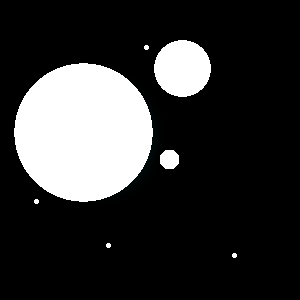
\includegraphics[height=3cm]{Images/morpho_init.png}
    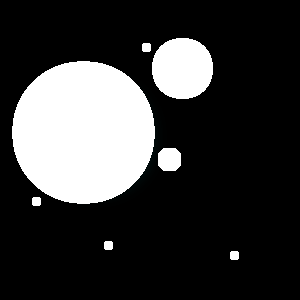
\includegraphics[height=3cm]{Images/morpho_dilate_k5.png}
    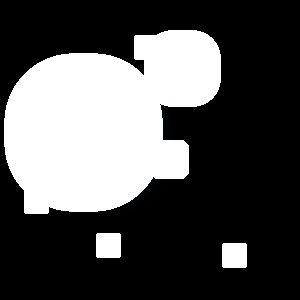
\includegraphics[height=3cm]{Images/morpho_dilate_k21.png}
    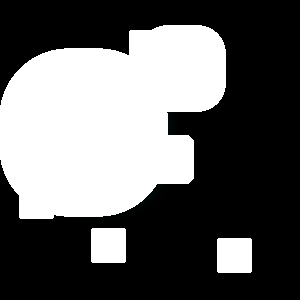
\includegraphics[height=3cm]{Images/morpho_dilate_k31.png}
    \label{fig:morpho_dilation}
    \caption{Exemple de dilatation}
  \end{figure}
  
  L'ensemble $B$ est couramment appelé \emph{élément structurant}.
  
  \paragraph{Érosion}
  
  L'opération opposée à la dilatation est l'érosion.
  
  \begin{equation}
    A \ominus B = \{x|(B)_x, \subseteq A\}
  \end{equation}
  
  L'érosion de $A$ par $B$ est l'ensemble de tous les points $x$ tel que $B$ translaté de x est inclus dans $A$. 
  
  \begin{figure}[h]
    \centering
    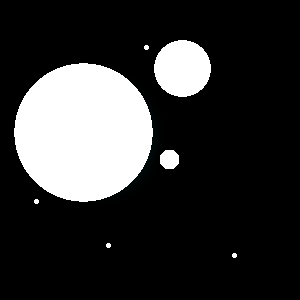
\includegraphics[height=3cm]{Images/morpho_init.png}
    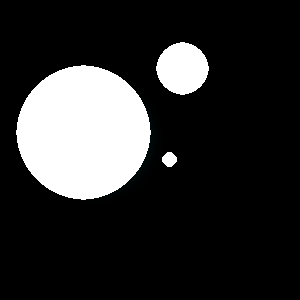
\includegraphics[height=3cm]{Images/morpho_erode_k5.png}
    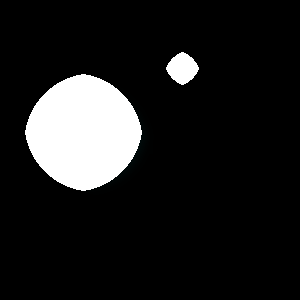
\includegraphics[height=3cm]{Images/morpho_erode_k21.png}
    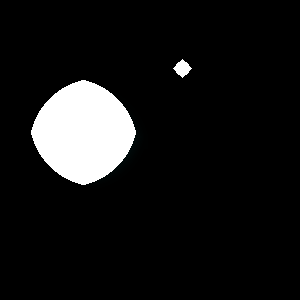
\includegraphics[height=3cm]{Images/morpho_erode_k31.png}
    \label{fig:morpho_erosion}
    \caption{Exemple d'érosion}
  \end{figure}
  
  \subsubsection{Fermeture et ouverture}
  
  À partir des opérations d'érosion et de dilatation, on peut définir des opérations composites : l'ouverture et la fermeture.
  
  \paragraph{Fermeture}
  L'ouverture est définie comme la dilatation de $A$ par $B$ suivi de l'érosion de $A$ par $B$.
  \begin{equation}
   A \bullet B = (A \oplus B) \ominus B
  \end{equation}
  
  Cet opérateur est utilisé pour boucher les trous dont la surface est inférieure à la surface de l'élément structurant. L'érosion qui suit la dilatation permet d'assurer que la taille reste stable.
  
  \begin{figure}[h]
    \centering
    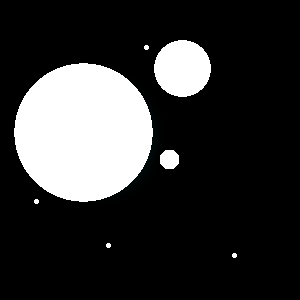
\includegraphics[height=3cm]{Images/morpho_init.png}
    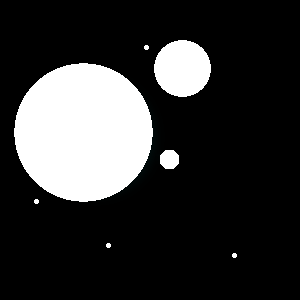
\includegraphics[height=3cm]{Images/morpho_close_k5.png}
    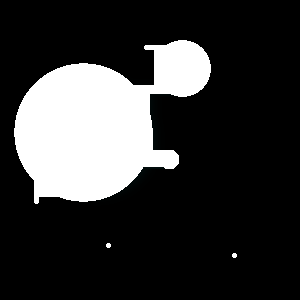
\includegraphics[height=3cm]{Images/morpho_close_k21.png}
    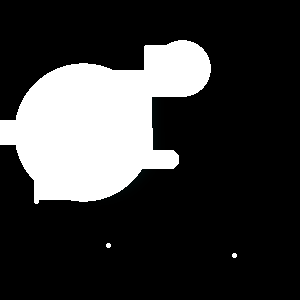
\includegraphics[height=3cm]{Images/morpho_close_k31.png}
    \label{fig:morpho_femerture}
    \caption{Exemple de fermeture}
  \end{figure}
  
  \paragraph{Ouverture}
  L'ouverture est définie comme l'érosion de $A$ par $B$ suivi de la dilatation de $A$ par $B$.
  \begin{equation}
   A \circ B = (A \ominus B) \oplus B
  \end{equation}
  
  \begin{figure}[h]
    \centering
    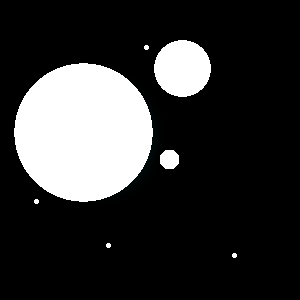
\includegraphics[height=3cm]{Images/morpho_init.png}
    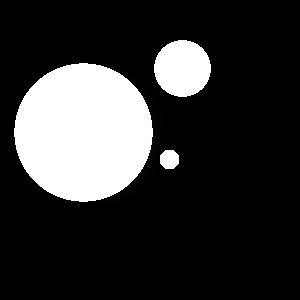
\includegraphics[height=3cm]{Images/morpho_open_k5.png}
    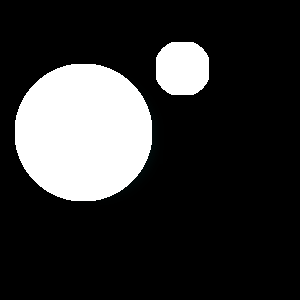
\includegraphics[height=3cm]{Images/morpho_open_k21.png}
    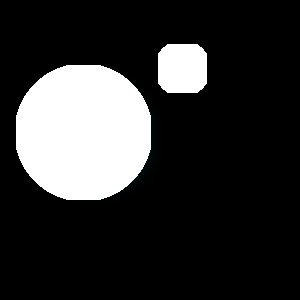
\includegraphics[height=3cm]{Images/morpho_open_k31.png}
    \label{fig:morpho_ouverture}
    \caption{Exemple d'ouverture}
  \end{figure}
  
  Cet opérateur est utilisé pour supprimer les structures de tailles inférieures à la surface de l'élément structurant. La dilatation qui suit l'érosion permet d'assurer que la taille des éléments restent stable.   L'ouverture permet de construire un espace d'échelle paramétré par la taille de l'élément structurant. Cet espace ne souffre pas d'une fusion parasite des structures adjacentes.
  
  \subsection{Flux}
  \label{sec:EA:rehaussement:echelle:flux}
  
  Comme nous l'avons vu dans la section SEC. \ref{sec:EA:rehaussement:echelle:gaussien}, l'espace d'échelle gaussien peut provoquer des débordements de structures sur d'autres, plus petites. On peut limiter ce problème en utilisant un cadre différent, celui de l'analyse des flux.
  
  Si l'on considère un champ de vecteur $V$, par exemple un fluide, ou un champ de gradient pour une image, on définit le flux passant à travers la surface $S$, orienté par sa normale $\vec{n_s}$, comme l'intégrale de la somme du produit scalaire entre le vecteur de flux $\vec{v}$ et la normale à la surface $\vec{n}$.
  
  \begin{equation}
  flux_S = \int_{S}< \vec{v},\vec{n} > d\rho
  \end{equation}
  
  On peut appliquer le calcul de flux à la surface d'un objet fermé. En particulier, des structures en forme de disques ou de sphères ont été particulièrement utilisées pour l'analyse de vaisseaux sanguins. On peut en effet contrôler directement le diamètre d'une sphère pour détecter les objets de la taille voulue. Cette formulation de l'échelle diffère des méthodes précédentes, car les objets tubulaires ne sont détectés que pour une échelle donnée, là où les deux autres techniques conservent les objets à l'échelle donnée et aux échelles supérieures. Elle a aussi l'avantage de limiter l'analyse du flux à la surface de la sphère et donc de produire une réponse qui ne déborde pas.
  
  La précision du calcul de l'intégrale de flux dépend du nombre d'échantillons effectués sur $S$. Plus celui-ci est grand, plus le calcul est coûteux. De plus, plus l'échelle sélectionnée est grande, et donc plus la surface de la sphère est grande, plus le nombre d'échantillons requis est important.
  
  Law propose une formulation élégante du calcul de flux dans le domaine de Fourier afin de réduire drastiquement le temps de calcul par rapport à l'implémentation naïve \cite{Law2009_efficient_implementation}.
  
  Pour y parvenir, Law propose d'exprimer le calcul de flux sous la forme d'une convolution dans le domaine temporel. L'avantage de la convolution est double, on évite l'étape d'échantillonage sur la surface et la convolution s'exprime comme une multiplication dans le domaine de Fourier. On peut exprimer le calcul de flux en terme de volume et non plus en terme de surface grâce au théorème de la divergence qui établit une égalité entre le flux à la surface d'un objet et le flux à l'intérieur de son volume. Ainsi :
  
  \begin{equation}
    flux_{\partial C} = \int_{\partial C}< \vec{v},\vec{n} > d\rho \equiv \int_{C }\Delta I d\nu
  \end{equation}
  
  Plus précisément :
  
  \begin{equation}
    f_s(x,y,z) = \int_{R_s}\vec{v}(x+t,y+p, z+q) . \vec{n}_{(t,p,q)}dA
  \end{equation}
  
  avec $R_s$ une région sphérique de rayon $s$; $dA$ une surface infinitésimale sur la surface $\partial R_s$; $\vec{n}_{(t,p,q)}dA$ le vecteur normal à $dA$ à la position $(t,p,q)$; et $\vec{v}$ le gradient de l'image $I$. $\vec{v}$ est obtenu à partir de l'image $I$ lissée par un noyau Gaussien afin d'assurer la dérivabilité du signal de $I$. $\vec{v}=\nabla(g*I)$.
  
  Qui est équivalent à :
  
  \begin{align}
    f_s(x,y,z) & = \int_{R_s} \vec{div}( \vec{v}(x+t,y+p, z+q) ) dtdpdq \\
    & = \int_{\omega} d_s(t,p,q) [\vec{div}( \vec{v}(x+t,y+p, z+q) )] dtdpdq
  \end{align}
  
  où $\omega$ est le domaine entier de l'image et $d_s(t,p,q)$ correspond à la fonction porte sphérique définie par :
  
  \begin{equation}
  d_s(x,y,z) = [\sqrt{x^2 + y^2 + z^2} \leq s]
  \end{equation}
  
  Ainsi, $f_s(x,y,z)$ peut être exprimé sous forme de convolution :
  \begin{align}
    f_s(x,y,z) & = \int_{\omega} d_s(t,p,q) [\vec{div}( \vec{v}(x+t,y+p, z+q) )] dtdpdq \\
               & = \int_{\omega} d_s(t,p,q) (\Delta(g*I(x+t,y+p, z+q)))] dtdpdq \\
               & = \int_{\omega} d_s(-t,-p,-q) (\Delta(g*I(x+t,y+p, z+q)))] dtdpdq \\
               & = d_s * \Delta g * I(x,y,z) \\
               & = I * h_s(x,y,z) \\
  \end{align}
  
  avec $*$ l'opérateur de convolution, $\Delta$ l'opérateur laplacien.
  
  Et dans le domaine de Fourier:
  
  \begin{align}
    FFT( I * h_s(x,y,z) ) &= FFT(I) . H_s(u,v,w) \\
                         &= FFT(I) . [ (j2 \pi)^2 ( (\frac{u}{N_x})^2 + (\frac{v}{N_y})^2 + (\frac{w}{N_z})^2 ) ] \\
                         & . [ exp( -( (\frac{u}{N_x})^2 + (\frac{v}{N_y})^2 + (\frac{w}{N_z})^2 ) 2(\pi\sigma)^2 ) ]
  \end{align}
  
  \begin{figure}[h]
    \centering
    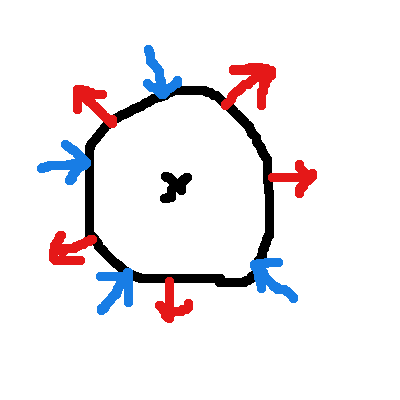
\includegraphics[height=6cm]{Images/flux.png}
    \label{fig:flux_sphere}
    \caption{flux sur la surface d'une sphère}
  \end{figure}
  
  \subsection{Multi-échelle}
  \label{sec:EA:rehaussement:echelle:multiScale}
  
  La combinaison de la détection de vaisseaux à plusieurs échelles est principalement fusionné grâce à un opérateur max effectué sur toutes les échelles.
  
  \begin{equation}
    V(I)_{multi echelle} = max_{\sigma}V_{\sigma}(I)
  \end{equation}
  
  Cet opérateur peut provoquer un recouvrement des structures adjacentes par une structure ayant une réponse plus haute. À notre connaissance, aucune publication ne propose de pondérer ou de hiérachiser la réponse en fonction de la taille du $\sigma$ (i.e. la taille des vaisseaux).


\section{Cactéristiques}


La différenciation entre les vaisseaux et d'autres structures s'effectue à l'aide de caractéristiques extraites de l'image qui permettent de définir localement la géométrie autour d'un pixel. 

\subsection{Morphologie}
\label{sec:EA:rehaussement:morpho}

Le rehaussement à base d'opérateurs morphologiques s'articule autour de deux familles, la composition d'éléments structurants rigides et l'utilisation de chemins curvilinéaires flexibles.

La composition d'éléments structurants rigides s'effectue la plupart du temps avec des boules et des cylindres. Les cylindres permettent de couvrir les parties curvilignes des vaisseaux, tandis que les boules couvrent les jonctions. Une composition d'ouvertures avec ces éléments est ensuite utilisée pour récupérer le réseau vasculaire. Sazak propose une schéma de ce type en 2 dimensions \cite{Sazak2019_bowler_hat_2D} puis en 3D \cite{Sazak2018_bowler_hat_3D} et compare son efficacité contre du rehaussement à base de tenseurs de phases et hessiens. Cette méthode bien que simple à mettre en pratique, nécessite plusieurs itérations avec des rotations des éléments structurants afin de capturer toutes les orientations des structures tubulaires. Cette méthode peut devenir coûteuse en 3D.

\begin{figure}[h]
  \centering
  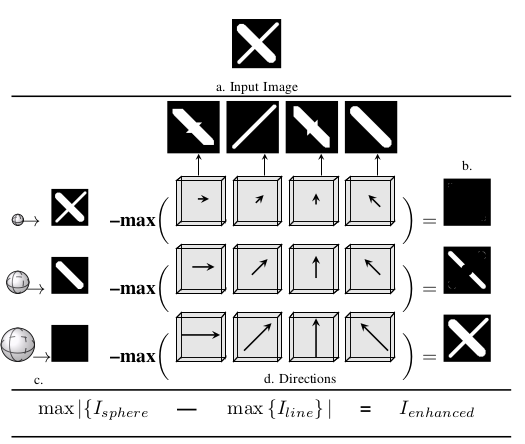
\includegraphics[height=4cm]{Images/bowlerHat_3D.png}
  \label{fig:sazak_bowler_hat}
  \caption{bowler hat transform proposée par Sazak et al. La combinaison d'éléments sphériques et linéaires permet de capture les structures curvilinéaires. }
\end{figure}

L'un des défauts de la méthode précédente est la rigidité des éléments structurants qui ne permettent pas toujours de capturer les variations de formes des vaisseaux. Hejimans \cite{Heijmans2005_path_opening} propose une famille d'éléments structurants flexibles dont la forme est définie par une grille d'adjacences. Des améliorations successives de cet algorithme ont été proposés : Cokelaer et al. \cite{Cokelaer2012_efficient_path_opening} propose une version robuste au bruit en autorisant des discontinuités dans l'élément structurant, Van de Gronde \cite{Gronde2015_fast_path_opening} propose une implémentation efficace de l'agorithm en $o( N log ( L ))$ avec $L$ la taille du chemin. Enfin Merveille et al. \cite{Merveille2018_curvilinear} itère sur la méthode en proposant un classement de l'orientation des chemins afin de segmenter les vaisseaux dans des images 2D et 3D (voir Sec. RORPO). 


\subsection{Phase}
\label{sec:EA:rehaussement:Phase}

Une image peut-être à la fois vue comme une matrice de pixels et comme un signal discret en 2 ou 3 dimensions. Lorsque l'on considère la représentation sous forme de signal on peut décomposer celui-ci en deux éléments indépendants : L'amplitude, correspondant à l'intensité des pixels et la phase, correspondant à la distance entre deux pics de deux signaux. La phase étant une mesure relative à la position des pics, elle ne prend pas en compte l'amplitude de ceux-ci et présente donc une invariance aux changements d'intensités. Oppenhei et al. \cite{Oppenheim1981_phase_importance} démontre l'importance de ces caractéristiques de l'image et montre une correspondance avec le système visuel humain. 

\begin{figure}[h]
  \centering
  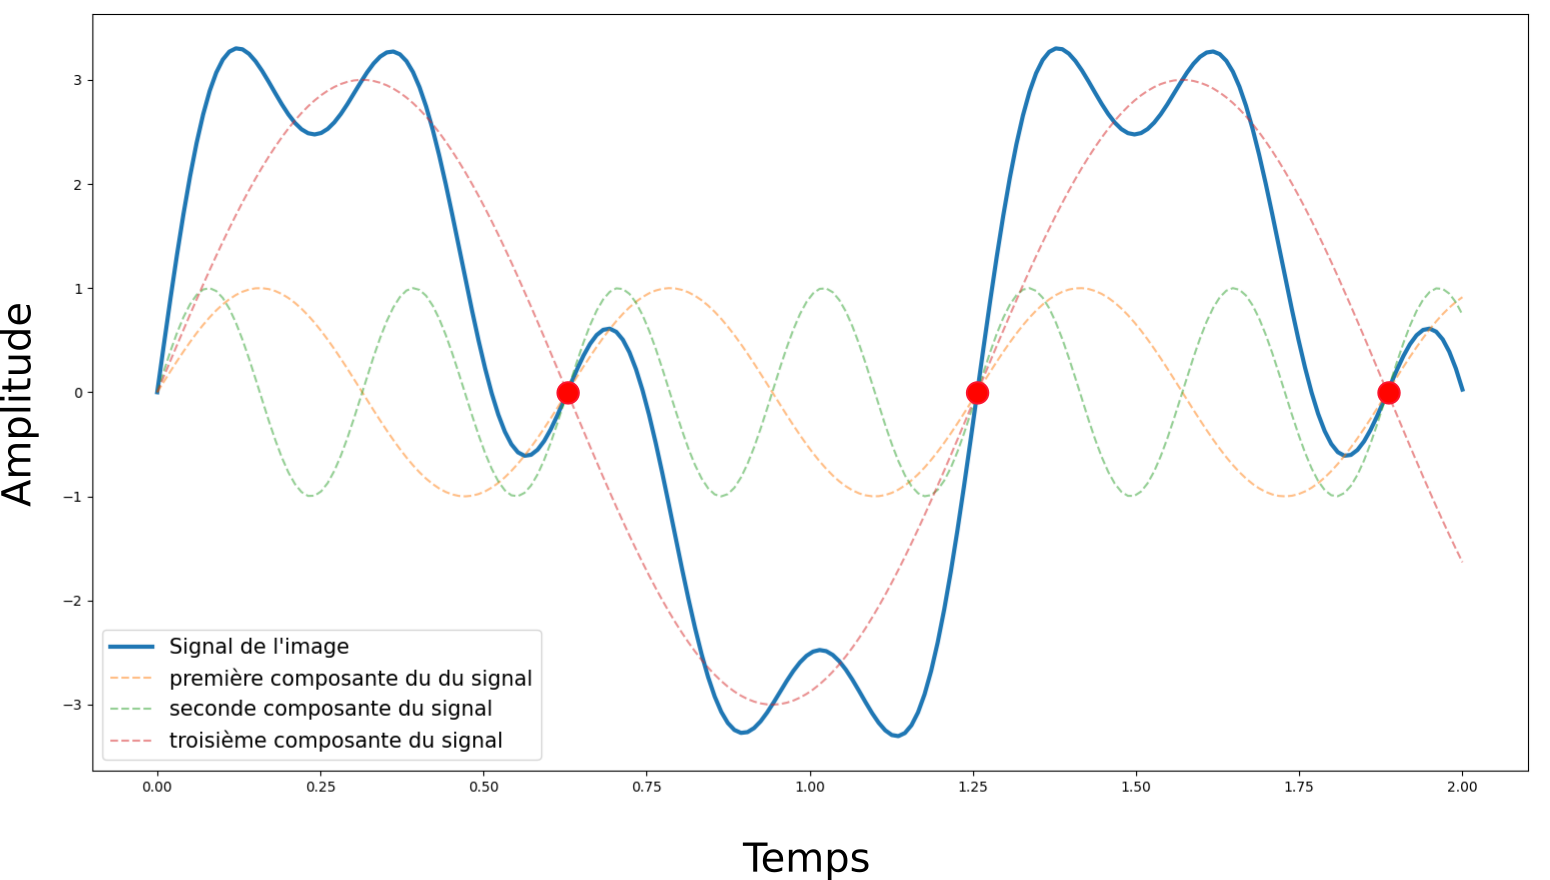
\includegraphics[height=5cm]{Images/PC_decomposition.png}
  \label{fig:phase congruency}
  \caption{Décomposition de Fourier d'un signal, en certains points la phase de chaque composant est synchronisée}
\end{figure}

Plusieurs constructions de filtres de rehaussement se basent sur cette propriété pour la détection des vaisseaux. Obara et al. \cite{Obara2012_phase} utilise un tenseur de structure basé sur le contraste de phase. Les valeurs propres de ce tenseur permettent ensuite d'exprimer une mesure de tubularité.

Ce tenseur est exprimé comme :

\begin{equation}
  T_{PC} = \sum PC_{o}(p)(n_{o}n^T - \alpha \text{I})
\end{equation}

Avec $PC(x)$ la fonction de congruence de phase, $n(\theta)=[cos(\theta),sin(\theta)]^T$ le vecteur d'orientation $o$,$\alpha = 1/(m-1)$ et $I$ le tenseur unitaire. $PC(x)$ permet de détecter les éléments saillants à la manière d'un détecteur de contours.
En effet, une image vue comme un signal peut être décomposée comme un ensemble de signaux sinusoïdaux. Les éléments saillants tels que les bordures ou les coins d'objets correspondent à une synchronisation, e.g congruence, de ces signaux pour un angle donné. Celle-ci s'exprime par :

\begin{equation}
  PC(x) = max_{\theta \in [0,2\pi)} \sum  \frac{ \alpha_{\omega}cos(\omega x + \phi_{\omega} - \omega)  }{ \alpha_{\omega}d \omega } d \omega
\end{equation}

Celle-ci représente la variance de phase des différents signaux au point $x$. Lorsque les phases des signaux sont égales $PC(x)=1$.
En pratique, cette définition est complexe à implémenter, on lui préfère en pratique la mesure d'énergie locale qui s'approxime avec des filtres de Gabor ou des ondelettes. Ces filtres sont basés sur des gaussiennes dont on peut contrôler l'échelle comme un espace gaussien.

\begin{figure}[h]
  \centering
  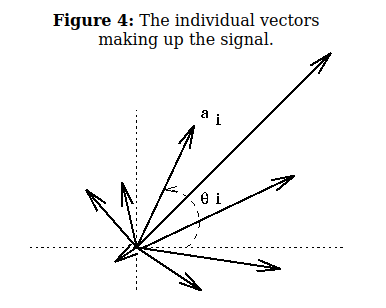
\includegraphics[height=5cm]{Images/PC_vectors.png}
  \label{fig:phase congruency}
  \caption{Représentation vectorielle d'un signal, chaque vecteur représente une composante sinusoïdale paramétrée par sa phase pour l'orientation et son amplitude pour sa norme}
\end{figure}

Enfin, ces filtres sont dépendants du nombre d'orientations échantillonnées $\omega$. En pratique entre 6 et 10 échantillons régulièrement espacés suffisent. 

\subsection{Hessienne}
\label{sec:EA:rehaussement:hessienne}

La matrice hessienne est la matrice des dérivées seconde de l'image en un pixel. Celle-ci permet d'exprimer la courbure locale autour d'un point.
Les valeurs propres et vecteurs propres de la Hessienne permettent de quantifier l'orientation, le sens et l'amplitude du voisinage d'un point.
La simplicité de la Hessienne a permis l'émergence de nombreuses modélisations de rehaussement.

En 3D, une structure tubulaire parfaite peut-être exprimée par les valeurs propres. Soit $\lambda_1$,$\lambda_2$,$\lambda_3$ tel que $|\lambda_1| \leq |\lambda_2| \leq |\lambda_3|$ alors un tube parfait est modélisée par :

\begin{align}
  \lambda_1 \approx 0 \\
  \lambda_1 \ll \lambda_2 \\
  \lambda_2 \approx \lambda_3
\end{align}

Ces équations sont valables dans un contexte spécifique. Lorsque le $\sigma$ de l'espace d'échelle coïncide avec la taille d'une structure tubulaire, la ligne centrale de celle-ci devient un maxima local. Le vecteur propre $\lambda_1 \approx 0$ correspond à la direction du tube. Dans ce cas, la magnitude $\lambda_1$ est proche de zéro car le gradient dans cette direction est presque nul. Dans les deux directions principales de la tranche, l'intensité du tube décroissant rapidement au fur et à mesure que l'on s'éloigne du centre, les valeurs propres $\lambda_2$ et $\lambda_3$ sont donc élevées.


\section{Mesures de tubularités}

Une des méthodes les plus communes de définir la tubularité est d'utiliser les valeurs propres de la Hessienne. Soit $e_1$, $e_2$ et $e_3$ les trois vecteurs propres de $H(f)$, associé aux valeurs propres $\lambda_1$,$\lambda_2$ et $\lambda_3$ tel que $|\lambda_1| \leqslant |\lambda_2| \leqslant |\lambda_3|$. En terme de valeurs propres, la tubularité peut s'exprimer de la manière suivante \cite{Lorenz1997_multi}:

\begin{align}
\nonumber
  |\lambda_1| & \approx 0 \\
\nonumber
  \lambda_2 \approx \lambda_3 & \ll 0
\end{align}

\subsection{Sato}

Sato \etal \cite{Sato1998_vesselness} est parmi les premiers à se servir de cette formulation. (N.B. : l'ordonnancement des valeurs propres est légèrement différent pour Sato $\lambda^\star_i$ tel que $\lambda^\star_1 \geqslant \lambda^\star_2  \geqslant  \lambda^\star_3$.)
Quand $\lambda^\star_2, \lambda^\star_3 < 0$, le vecteur propre $\mathbf {e^\star_1}$ associé à $\lambda^\star_1$ pointe dans la direction de la plus petite variation d'intensité, qui est aussi la direction du vaisseau.
Dans ce cas les vecteurs propres $\mathbf {e^\star_2}$ et $\mathbf {e^\star_3}$ forment une base orthogonale à $\mathbf {e^\star_1}$ et correspondent à la tranche du vaisseau.
La taille des axes de la tranche des vaisseaux est proportionnelle à $|\lambda^\star_2|$ et $|\lambda^\star_3|$.

Le filtre de rehaussement de Sato utilise un ratio asymétrique de valeurs propres pour obtenir une réponse forte sur les structures tubulaires, basé sur le signe de $\lambda^\star_1$.
Ce filtre à l'avantage de lisser la réponse et de réduire le bruit. Deux paramètres $\alpha_1$ et $\alpha_2$ contrôlent la force de cette asymétrie:
\begin{equation}
\nonumber
F =
\left\{
\begin{array}{lr}
\lambda^\star_c \exp(-\frac{{\lambda^\star_1}^2}{2(\alpha_1 \lambda^\star_c)^2})  & \lambda^\star_1 \leqslant 0, \lambda^\star_c \neq 0 \\
\lambda^\star_c \exp(-\frac{{\lambda^\star_1}^2}{2(\alpha_2\lambda^\star_c)^2})  &  \lambda^\star_1 > 0, \lambda^\star_c \neq 0 \\
0 & \quad \lambda^\star_c = 0
\end{array}
\right.
\end{equation}
avec $\lambda^\star_c = \min\{-\lambda^\star_2,-\lambda^\star_3\}$.

\subsection{Frangi}

Une année plus tard, Frangi \etal \cite{Frangi1998_vesselness} exploite l'ensemble des valeurs propres afin de proposer un contrôle plus fin sur la géométrie des motifs rehaussés. Trois mesures sont dérivées des valeurs propres :

\begin{align}
 \nonumber
  R_b & = |\lambda_1| / \sqrt{|\lambda_2\lambda_3|}\\
R_a & = |\lambda_2| / |\lambda_3| \nonumber\\
S & = \sqrt{\lambda^2_1 + \lambda^2_2 + \lambda^2_3} \nonumber
\end{align}

Ces mesures permettent de discriminer les blobs ($R_b$), différencier les plateaux des structures en ligne ($R_a$) et de contrôler les structures de faible contraste en étudiant la norme de la Hessienne ($S$). C'est trois mesures sont unifiée dans une fonction de rehaussement :   

\begin{equation}
\nonumber
  F =
   \big(1-\exp\big(-\frac{R_a^2}{2\alpha^2}\big)\big) \exp\big(-\frac{R_b^2}{2\beta^2}\big)\big(1-\exp(-\frac{S^2}{2C^2}\big)\big)
\end{equation}
if $\lambda_2, \lambda_3 \leqslant 0$ et $F = 0$ sinon.

Cette fonction est contrôllée par trois paramètres $\alpha$, $\beta$, $C$, faisant du filtre de Frangi le filtre nécessitant le paramétrage le plus demandeur. Cette méthode est utilisé dans la plupart des applications de segmentation avec rehaussement.

\subsection{Meijering}

Meijering \etal \cite{Meijering2004_neurite_vesselness} propose un filtre pour la détection de neurites dans des images fluoroscopiques. Il s'intéresse en particulier à rehausser les structures fines de un ou deux voxels de large. Cette méthode est sans parmaètres et a été initialement proposée en 2D; Elle a ensuite été testée en 3D dans \cite{Obara2012_phase}. Cependant, en 3D une formulation n'a jamais été explicitement documenté, ce que nous clarifions en annexe (Anex. \ref{APP:Proof of Meijering's maximal flatness for 3D case}). Le filtre repose sur une matrice Hessienne modifiée H'(f) que nous définissons de la manière suivante :

\begin{equation}
  %\small
    \begin{bmatrix}
    \alpha h_{11}+ h_{22} +   h_{33} ~~~~~~~~~ h_{12} ~~~~~~~~~~~~~~~~~~~~~~~~~ h_{13} ~~~~~~~~ \\
    h_{21} ~~~~~~~~~~~~ \alpha h_{22} + h_{11} +  h_{33} ~~~~~~~~~~~~~~ h_{23} \\
    ~~~~~~ h_{31} ~~~~~~~~~~~~~~~~~~ h_{32} ~~~~~~~~~~~~~~ \alpha h_{33} + h_{11} +  h_{22}
    \end{bmatrix}
  \end{equation}

Le paramètre $\alpha$ est utilisé pour orienter le filtre afin que sa crête soit plate de manière maximale dans une direction, qui est obtenu quand $\alpha=-2/3$. Les trois valeurs propres de $H'(f)$ sont exprimées en fonctions de celles de $H(f)$ comme :

\begin{equation}
  \begin{aligned}
    \nonumber \lambda_1' = \alpha\lambda_1 + \lambda_2 + \lambda_3 \\
    \nonumber \lambda_2' = \lambda_1 + \alpha\lambda_2 + \lambda_3 \\
    \nonumber \lambda_3' = \lambda_1 + \lambda_2 + \alpha\lambda_3
  \end{aligned}
\end{equation}
for $i \neq j \neq k \neq i$.
La mesure de tubularité est alors :
\begin{equation}
\nonumber 
  F =
  \left\{
  \begin{array}{lr}
    \lambda_{\max} / \lambda_{\min}   &  \lambda_{\max} < 0\\
      0 &  \lambda_{\max} \geqslant 0
  \end{array}
  \right.
\end{equation}

Où $\lambda_{max} = max\{\lambda_{1}^{'},\lambda_{2}^{'},\lambda_{3}^{'}\}$ est calculé pour chaque voxel, et $\lambda_{min}$ est la valeur propre minimale parmi toutes les valeurs propres de l'image.

\subsection{OOF}

N'importe quelle fonction peut-être utilisée dans le cadre de OOF. Pour ce banc de test, nous avons sélectionné la moyenne géométrique utilisée par ses auteurs dans leur expérience sur des données réelles :

\begin{equation}
\nonumber
    F =
    \left\{
    \begin{array}{lr}
    
    \sqrt{|\lambda_2 \cdot \lambda_3|}   & \lambda_2, \lambda_3 < 0 \\
    0     & \textrm{otherwise}
    \end{array}
    \right.
\end{equation}

\subsection{Jerman}

Jerman \etal a proposé une fonction de rehaussement dont l'objectif est de renforcer le signal aux bifurcations tout en proposant un filtre plus simple à paramétrer. Le rehaussement proposé repose sur la mesure volume aspect ratio, utilisé pour détecter des tenseurs presque sphériques. La fonction est définie par :

\begin{equation}
\nonumber
  F =
\left\{
  \begin{array}{lr}
    0 & \lambda_2 \leqslant 0 \textrm{~or~} \lambda_\rho \leqslant 0 \\
    1 & \lambda_2 \geqslant \lambda_\rho / 2 > 0 \\
    \lambda_2^2(\lambda_\rho -\lambda_2)\big(\frac{3}{\lambda_2+\lambda_\rho}\big)^3 & \textrm{otherwise}
  \end{array}
  \right. 
\end{equation}

Où $\lambda_\rho$ est la version régularisée du paramètre $\lambda_3$, défini pour réduire la sensibilité du filtre aux régions peu contrastées :
\begin{equation}
\nonumber
  \lambda_\rho =
  \left\{
  \begin{array}{lr}
     \lambda_3  & \lambda_3 > \tau \max_{x} \lambda_3(x) \\
    \tau \max_{x} \lambda_3(x) & 0 < \lambda_3 \leqslant \tau \max_{x} \lambda_3(x) \\
    0  & \textrm{otherwise}
  \end{array}
\right.
\end{equation}
Avec $\tau \in [0,1]$. Cette paramétrisation produit une réponse du filtre plus homogène, même pour des vaisseaux avec profils non-homogènes.

\subsection{Zhang}

Zhang et al. propose d'améliorer le rehaussement de Jerman dans le contexte de la segmentation de vaisseaux hépatiques, et plus particulièrement sur le foie maqué. Pour résoudre ce problème de réponses fortes sur les bords du foie, les auteurs proposent une classification à base de K-moyennes pour estimer les intensités moyenne des vaisseaux. Ils utilisent ensuite ces intensités moyennes pour paramétrer une fonction sigmoïd pour filtrer les autres tissues. De plus, ils modifient légèrement le rehaussement de Jerman $F$ en ajoutant un terme multiplicatif $terme$.

N'importe quelle fonction peut-être utilisée dans le cadre de OOF. Pour ce banc de test, nous avons choisis la moyenne géométrique utilisée par ses auteurs dans leur expérience sur des données réelles :

\begin{equation}
\nonumber
    F =
    \left\{
    \begin{array}{lr}
    
    \sqrt{|\lambda_2 \cdot \lambda_3|}   & \lambda_2, \lambda_3 < 0 \\
    0     & \textrm{otherwise}
    \end{array}
    \right.
\end{equation}

\subsection{RORPO}

RORPO \cite{Merveille2018_curvilinear} est construit sur l'espace d'échelle définit par l'ouverture de chemins. Pour capturer les structures curvilinéaires, les éléments structurants sont définis comme des chemins sur une grille d'adjacence qui fournit un cadre flexible sur la géométrie des éléments à détecter. Les ouvertures sont calculées avec des éléments structurants définis dans 7 orientations de l'espace 3D de manière à capturer les objets de différentes formes tel que les blobs, les structures linéaires et les plateaux. Une étape finale consiste à classifier les différentes formes en classifiant les orientations des éléments structurants. En effet, pour des objets tubulaires, tous les éléments structurants sont orientés dans la même direction.


\section{Diffusion}
\label{sec:EA:rehaussement:diffusion}

Les méthodes de diffusions sont une classe un peu à part dans le rehaussement des vaisseaux. L'objectif des frameworks de diffusion est d'améliorer le signal des vaisseaux en homogénéisant leur intensité et en renforçant leurs bordures. Pour cela, les filtres de diffusion proposent un schéma de lissage itératif qui prennent en compte la géométrie des structures à lisser.

HDCS \cite{Mendrik2009_HDCS} (Hybrid diffusion with continuous switch), propose un lissage hybride combinant lissage isotropique de régions et lissage basé sur les bordures. Ces deux lissages sont combinés avec une mesure de la géométrie locale afin d'appliquer une combinaison linéaire des deux filtres la plus adaptée.

VED \cite{Manniesing2006_VED} (Vessel enhancement diffusion)propose un lissage basé sur les méthodes de rehaussement Hessiens. Ce cadre permet ainsi d'homogénéiser la réponse de n'importe quel filtre de rehaussement Hessien en lissant selon le sens du rehaussement.

Ces méthodes itératives sont coûteuses en temps de calcul et nécessitent une paramétrisation supplémentaire pour contrôler la force du lissage ainsi que le nombre d'itérations nécessaire.

\section{Bilan et orientation des travaux}
\label{sec:EA:bilan}

Les constatations émises après l'état de l'art de la segmentation sont sensiblement les mêmes pour le rehaussement de vaisseaux. Les articles originaux testent souvent leurs méthodes sur des structures synthétiques simples ou des exemples variés. Elles sont toujours testées contre 2 à 4 autres méthodes. Lorsqu'ils sont utilisés sur des données réelles, les filtres de rehaussement sont largement utilisés avec les paramètres recommandés par l'auteur, sans adaptation à une application particulière.

Quelques travaux portent sur la comparaison des filtres de rehaussement. Luu et al. \cite{Luu2015_liver_vesselness_comparison} propose une comparaison de 3 filtres de rehaussement et 3 filtres de diffusion pour la tomodensitométrie du foie. Phellan et al. \cite{Phellan2017_Brain_vesselness_comparison} propose une comparaison de 6 filtres de rehaussement et 3 filtres de diffusions pour l'IRM du cerveau et un jeu de données synthétique.

Cependant ces travaux ne nous permettent pas de répondre à plusieurs questions :

\begin{itemize}
\item Quel filtre utiliser pour l'IRM du foie ?
\item Quel est l'impacte de la paramétrisation sur la réponse des filtres ?
\item Quels types de vaisseaux sont le mieux rehaussés ?
\item Quel est l'impacte des filtres de rehaussement indépendamment de la segmentation ?
\end{itemize}